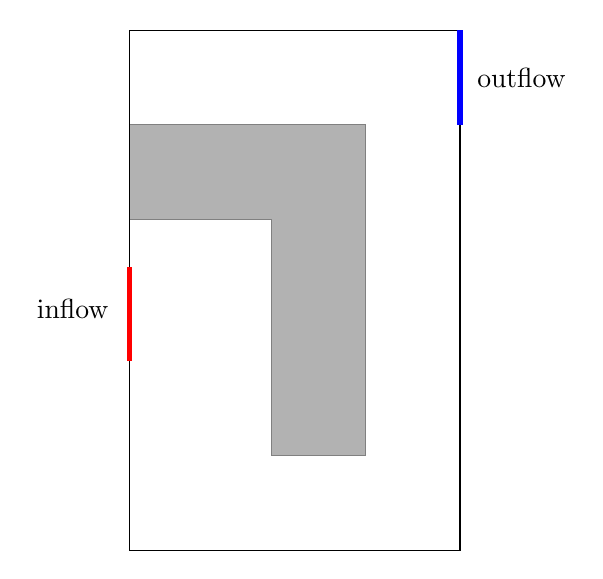
\begin{tikzpicture}
[scale=0.6]
% obstruction
\filldraw[fill=black!30,draw=black!50](3,2) -- (5,2) -- (5,9) -- (0,9) -- (0,7) -- (3,7) -- (3,2) ;
% domain
\draw (0,0) -- (7,0) -- (7,11) -- (0,11) -- (0,0);
% inflow
\draw [draw=blue, line width=2 pt] (7,9) -- (7,11);
\draw (8.3,10) node {outflow};
% outflow
\draw [draw=red, line width=2 pt] (0,4) -- (0,6);
\draw (-1.2,5.1) node {inflow};
\end{tikzpicture}
%\\ \centering {Geometrie}
%

